\chapterhead{5}{Testing a Model}{Comparing what it predicts with the real thing}\label{ch5}

A model earns trust by being tested. Ask it a question, write the answer \emph{before} measuring, then measure the real thing and compare. The difference is a \textbf{gap}. A small gap is good, but how small is small enough depends on the question.

\begin{center}
\sffamily\small\renewcommand{\arraystretch}{1.5}
\begin{tabular}{@{}p{3.4cm}p{3.7cm}p{3.7cm}@{}}
\toprule
\textbf{Model} & \textbf{What it keeps} & \textbf{What it drops}\\
\midrule
A prediction & what the model says & how sure we should be\\
A gap & how far off the model was & why it was off\\
A margin & how much room a question has & the model's own errors\\
\bottomrule
\end{tabular}
\end{center}

\begin{tryit}{Predict, then check}
Use your $1:50$ model. Choose three distances in the room. For each, measure it on the model, multiply by 50 for a prediction, and then measure the real distance. Work out the gap.\par\medskip
\renewcommand{\arraystretch}{1.6}
\begin{tabular}{|p{3.4cm}|c|c|c|}
\hline
\textbf{Distance} & \textbf{Model says (cm)} & \textbf{Real (cm)} & \textbf{Gap (cm)}\\ \hline
 & & & \\ \hline
 & & & \\ \hline
 & & & \\ \hline
\end{tabular}
\end{tryit}

\begin{worked}{Practice numbers, not from a real room}
Bed to door: model 3.2~cm, so 160~cm. Real 164~cm. Gap 4.\\
Bed length: model 4~cm, so 200~cm. Real 200~cm. Gap 0.\\
Desk end to wall: model 1.2~cm, so 60~cm. Real 58~cm. Gap 2.\\
The biggest gap is 4~cm.
\end{worked}

\begin{center}
\begin{tikzpicture}
  \node[bigcir,minimum size=2.4cm] (a) at (0,0) {}; \node[font=\sffamily\scriptsize,align=center] at (0,0) {model\\160};
  \node[cir] (b) at (4,0.9) {164}; \node[cir] (c) at (4,-0.9) {4};
  \draw[popA] (a) -- node[above,note] {real} (b); \draw[popA] (a) -- node[below,note] {gap} (c);
  \node[note,anchor=west,text width=2.8cm,align=left] at (5.0,0) {$164-160=4$};
\end{tikzpicture}
\end{center}

\begin{multix}[hmm]\multixbot[hmm]\tcblower
The gaps are 4, 0 and 2~cm, which are tiny. So the model is correct and good for every question. I will now use it to fit a chair 59~cm wide into a gap of 60. Safe?
\end{multix}

\trust{We wrote each prediction before measuring, then measured the real room and worked out every gap.}
{The three gaps were all 4~cm or less, so the model can answer questions with a margin of more than about 5~cm.}
{Questions with a smaller margin. A 4~cm gap is nothing for a bed and a lot for a chair squeezed into a narrow gap.}

\begin{keepbox}
We turned a model into predictions and gaps. \textbf{We kept} \wline[3.4cm] \textbf{and we set aside} \wline[3.4cm].
\end{keepbox}

\begin{tryit}{Check the margin}
A \textbf{margin} is the spare room a question has. Pick things to fit into gaps in your room and write the margin for each. A model can be trusted for a question when the margin is bigger than its biggest gap.\par\medskip
\renewcommand{\arraystretch}{1.6}
\begin{tabular}{|p{3.1cm}|c|c|c|c|}
\hline
\textbf{Thing in gap} & \textbf{Thing (cm)} & \textbf{Gap (cm)} & \textbf{Margin} & \textbf{Safe?}\\ \hline
 & & & & \\ \hline
 & & & & \\ \hline
\end{tabular}
\end{tryit}

\begin{worked}{Practice numbers}
Basket 40~cm in a 60~cm gap: margin 20, bigger than 4, safe.\\
Chair 59~cm in a 60~cm gap: margin 1, smaller than 4, not safe.\\
Bed 200~cm in a 190~cm gap: margin $-10$. The bed does not fit, and 10 is bigger than 4, so the answer ``no'' is safe.
\end{worked}

\clearpage

\begin{puzzle}{Find the gap}
Model says 160~cm and real is 164~cm. The gap is \wline[1.6cm]~cm.
\end{puzzle}

\begin{puzzle}{Predict}
A model distance is 2.6~cm at $1:50$. Predict the real distance. \wline[1.6cm]~cm
\end{puzzle}

\begin{puzzle}{Margin}
A basket is 40~cm and the gap is 60~cm. Margin \wline[1.6cm]~cm. Safe if the biggest gap is 4~cm? \wline[2cm]
\end{puzzle}

\begin{puzzle}{Tight fit}
A chair is 59~cm and the gap is 60~cm. Margin \wline[1.6cm]~cm. Safe? \wline[2cm]
\end{puzzle}

\begin{puzzle}{Safe ``no''}
A bed is 200~cm and the gap is 190~cm. The model says it does not fit. Is that answer safe? \wline[2cm] Why? \wline[4cm]
\end{puzzle}

\clearpage

\begin{puzzle}{Why three?}
Why test a model on three predictions and not just one? \wline[6cm]
\end{puzzle}

\begin{puzzle}{Unfair test}
Ana measured the model with a ruler and the real room with a tape, then wrote down only the one gap that was zero. What is wrong? \wline[6cm]
\end{puzzle}

\begin{puzzle}{Draw the circles}
Model says 60, real is 58. Draw the circles for the model, the real value and the gap.
\begin{center}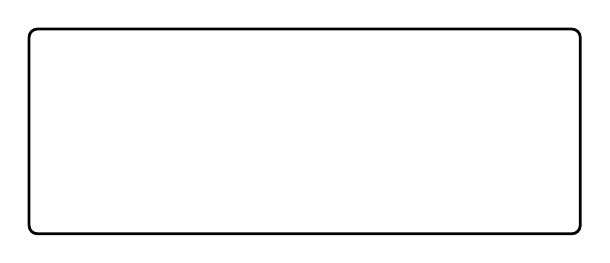
\begin{tikzpicture}\draw[line width=1pt,rounded corners=3pt] (0,0) rectangle (7,2.6); \end{tikzpicture}\end{center}
\end{puzzle}

\begin{puzzle}{Wrap}
A student wrote ``The model is correct.'' Wrap it with a better claim. \wline[6cm]
\end{puzzle}

\begin{puzzle}{Design a test}
Plan a test of your own model and say which question you will ask it. \wline[6cm]
\end{puzzle}
\clearpage

\thispagestyle{fancy}
\subhead{Prediction record}
Test your model on five predictions.\par\medskip
\renewcommand{\arraystretch}{2.8}
\begin{tabularx}{\linewidth}{|>{\sffamily\small\bfseries}p{2.4cm}|X|X|X|X|}
\hline
Distance & Model says & Real & Gap & Margin of question \\ \hline
 & & & & \\ \hline
 & & & & \\ \hline
 & & & & \\ \hline
 & & & & \\ \hline
 & & & & \\ \hline
\end{tabularx}

\vspace{8pt}
What is your biggest gap? \wline[7cm]\\[10pt]
For what size of question can you trust your model? \wline[5cm]\\[10pt]
Draw your gaps as a bar chart.\par\medskip
\begin{tikzpicture}\draw[ink!70,line width=1pt,rounded corners=3pt] (0,0) rectangle (11.4,4.2);\end{tikzpicture}
\clearpage
